
%• What did you personally contribute to the project?

%The project report should stand on its own (i.e., it should not assume familiarity with your project or with your planning paper), but you may reuse material from your previous paper if you want. It is both a report on what you did, as well as a reflection of what you learned in your project.

\documentclass[11pt,a4paper]{article}
\usepackage[hyperref]{acl2018}
%\usepackage{fancyhdr}
%\aclfinalcopy % Uncomment this line for the final submission
%\def\aclpaperid{***} %  Enter the acl Paper ID here

%\setlength\titlebox{5cm}
% You can expand the titlebox if you need extra space
% to show all the authors. Please do not make the titlebox
% smaller than 5cm (the original size); we will check this
% in the camera-ready version and ask you to change it back.

\usepackage{amsmath} % mathematical notation
\usepackage{amsfonts} % for number sets
\usepackage{graphicx} % for imports
\usepackage{subcaption} % for figures
\usepackage{cleveref} % better references
\usepackage{csquotes} % enquote
%\usepackage[mode=buildnew]{standalone}
\usepackage[shortlabels]{enumitem}
\graphicspath{{../../data/img/}}
\usepackage{pgfplots} % plotting pgf format directly
% citations

\usepackage{adjustbox}
\title{Project Report}

\author{Luis Glaser\\
  registration number 800140 \\
  Potsdam University \\
  {\tt Luis.Glaser@uni-potsdam.de} \\
  \\
  Advanced Natural Language Processing (WS 2018/2019) \\
  Dr. Tatjana Scheffler \\
  \\}

\date{01. March 2019}
\usepackage{url}
\makeatletter
\tikzset{
    database/.style={
        path picture={
            \draw (0, 1.5*\database@segmentheight) circle [x radius=\database@radius,y radius=\database@aspectratio*\database@radius];
            \draw (-\database@radius, 0.5*\database@segmentheight) arc [start angle=180,end angle=360,x radius=\database@radius, y radius=\database@aspectratio*\database@radius];
            \draw (-\database@radius,-0.5*\database@segmentheight) arc [start angle=180,end angle=360,x radius=\database@radius, y radius=\database@aspectratio*\database@radius];
            \draw (-\database@radius,1.5*\database@segmentheight) -- ++(0,-3*\database@segmentheight) arc [start angle=180,end angle=360,x radius=\database@radius, y radius=\database@aspectratio*\database@radius] -- ++(0,3*\database@segmentheight);
        },
        minimum width=2*\database@radius + \pgflinewidth,
        minimum height=3*\database@segmentheight + 2*\database@aspectratio*\database@radius + \pgflinewidth,
    },
    database segment height/.store in=\database@segmentheight,
    database radius/.store in=\database@radius,
    database aspect ratio/.store in=\database@aspectratio,
    database segment height=0.1cm,
    database radius=0.25cm,
    database aspect ratio=0.35,
}
\makeatother
%========================================================
% BEGIN DOCUMENT
%========================================================
\begin{document}
\maketitle


%\pagestyle{fancy}
\section{Introduction}\label{sec:introduction}
Together with Atreya Shankar and Juliane Hanel I worked on music lyrics. The original motivation was our shared interest in music and the different social and political dimension that can be expressed through it. Although music also consists of the audio signal, lyrics do play an important role when analyzing. E.g. \citet{DBLP:conf/coling/FellS14} noted, that considering lyrics in recommendation engines does increase their quality.

%========================================================
% SUMMARY
%========================================================
This final paper will be split in two major parts: First, I will elaborate our method, lay out our results and point out our findings. Notice that I will focus mostly on the technical background, since that was the focus of my contribution.

The second large part in \cref{sec:reflection} will be focussed on the project's effects, how I contributed to it and what I learned from it. 
\paragraph{Definitions}\label{sec:definitions}

Throughout this paper, I will discuss significance of changes. I will use standard asterisk abbreviations for the magnitude of the p-values: $* := p \leq .05,\ ** := \leq .01,\ *** := \leq .001$.

Since our data set has a high number of entries ($23,135$ songs in final dataset), we looked at effect size measures as well \citep{Psychdict}.
We use the dagger symbol to signify those: $\dagger := d \geq 0.2$.

For easier analysis and due to uneven data (more detail in \cref{sec:scraping}) we binned our data in three time ranges:
$T_1 = [1970,2000]$. $T_2 = (2000,2010]$ and $T_3 = (2010,2019]$.
%========================================================
% What was the topic of your group’s project, your approach and main results?
%========================================================

%\section{Project documentation}\label{sec:documentation}

\section{Hypotheses}\label{sec:hypotheses}

To work on more concrete topics, we initially agreed on three hypothesis we wanted to focus on. These were:

\begin{enumerate}[$H_1$]
	\item \label{hypo:country} Country music has incorporated mainstream Pop music features.
	\item \label{hypo:ego} Pop music became more egocentric. 
	\item \label{hypo:lexical} Popular music of all genres became less lexically diverse. 
	
\end{enumerate}

%========================================================
% METHOD
%========================================================

\section{Method}\label{sec:method}

Bearing these hypotheses in mind, this section will elaborate on how we collected our data (\Cref{sec:scraping}), what annotations we applied (\Cref{sec:annotations}) and what metrics we used to test our hypotheses (\Cref{sec:metrics}). 
\subsection{Scraping}\label{sec:scraping}

We initially planned, to use data from a kaggle competition \citep{kuznetsov_55000+_2017} for our analysis. However, it contained a significant bias to one specific year, as shown in \cref{fig:histograms:kaggle}. We thus decided to create the dataset on our own, using the popular site \url{genius.com}. There, users can create entries for lyrics by themselves and annotate them collaboratively.

\begin{figure}[t!]
\begin{adjustbox}{width=0.5\textwidth}
    \begin{tikzpicture}[line width=1pt]
% Nodes
\node[inner sep=0pt] (wiki) at (0,6)
    {\includegraphics[width=2cm]{wikipedia-logo-en.png}};
\node[database,label=below:\texttt{SQLite3},database radius = 0.75cm, database segment height = 0.3cm] (db) at (2,0) {};

\draw[->,line width=2,draw=blue!50] (wiki.south) to [out=265,in=160] (db);
\node[inner sep=.1cm, align=center,fill=white] (expArtistlist) at (-1.3,4) {(1) scrape artist names \\ per genre};

\node[] (genius) at (6,6)
	{\Large \texttt{www.genius.com}};

\draw[->,line width=2,draw=blue!50] (db.east) to [out=0,in=280](genius.south);
\node[inner sep=.1cm, align=center,fill=white] (expArtistlist) at (6,3) {(2) query artist name};

\draw[->,line width=2,draw=blue!50] (genius.west) to [out=220,in=90] (db.north);
\node[inner sep=.1cm, align=center,fill=white] (expArtistlist) at (2.5,2.25) {(3) store lyrics \& metadata};
\end{tikzpicture}
\end{adjustbox}
    \caption{Breakdown of data-scraping methodology using Wikipedia and the Genius API}	
    \label{fig:scrape}
\end{figure}

Since the \url{genius.com}-API does not offer a \emph{wildcard-search}, we had to collect names of artists ourselves. Our approach is sketched in \cref{fig:scrape}. 

(1) We used wikipedia, more specifically the \enquote{List of [...] artists} lists, that can be found for a variety of different genres. There, we extracted artist names with simple \texttt{regex} rules and stored them to our \texttt{SQLite3}-backed database. 

(2) Then, we queried genius using the \texttt{requests}-package for these artists names. 
Unfortunately, the API always returns songs, represented by a \texttt{json}-object, except when querying for an artist id directly. To obtain these, we used a work-around: When the name of the primary artist in a returned song-\texttt{json} equals the artist we queried for, we found their internal id. With that, we can then directly query the urls of their songs. 

(3) From these sites we could then scrape lyrics and publication year directly using \texttt{BeautifulSoup4}. This might seem to be a cumbersome approach, however genius is one of the most prominent sites and despite throtteling the request rate at some point, they do not block IPs querying a lot of data. %TODO example und cite lyricswikia bug

With this approach, we were able to at least reduce the temporal bias compared to the kaggle data (cf. \cref{fig:histograms:genius}). But, we still had spikes in \emph{round} years (e.g. 2010 and 2000). Potentially when an annotator was unsure in which year exactly a song was published they simply entered the decade. Bear in mind, genius data is user generated. Thus, we decided to bin our data for most analysis into the three bins $T_1, T_2$ and $T_3$ as described in \cref{sec:definitions}.


\Cref{tab:scrape:idscomp} shows an overview of artists that we collected from wikipedia and in turn how many we were able to find on genius. We can directly see a significant drop. This drop stems from multiple factors: Annotations in artist names on wikipedia ( \enquote{Torch (American)} and \enquote{Torch (German)}), bad encoding (\enquote{Cam'ron} being resolved as \enquote{Cam\%27ron}) or simple name missmatches (\enquote{B.o.B} on wikipedia, \enquote{BoB} on genius). Also, to save computation time, we only queried 20 results in search of an artist ID (Step 2). This could result in returning song titles instead of artists before we could get a match, when artist names were common English words that could occur in titles (e.g. \enquote{Future}, \enquote{Bohemia} or \enquote{Choice}).

\begin{table}[t!]
\begin{tabular}{llll}
\hline
Genre & Wikipedia & genius ID & drop \\ \hline 
Country & $1969$ & $1237$ & 0.39 \\
Pop & $683$ & $349$ & 0.49 \\
Hip Hop & $1370$ & $866$ & 0.37 \\ \hline
\end{tabular}
\caption{Artist change between wikipedia and genius}
\label{tab:scrape:idscomp}
\end{table}
\subsection{Annotation}\label{sec:annotations}

In order to test the hypotheses enumerated in \cref{sec:hypotheses} and draw conclusions from them, we needed to clean and annotate our data in multiple ways. This section will layout this process and illustrate each of elements of our pipeline. 

All annotations below will be defined w.r.t a document $d$ which denotes the lyrics of one song. A document with length $n$ contains a range of words $(w_0, \ldots, w_n)$. 
\paragraph{Language Recognition}

We limit our work on English lyrics. First, since the large majority of lyrics collected are English. Second, since including tooling for other languages was beyond the scope of this work. For this process we used the python package \texttt{lang-detect} \citet{danilak_lang_2017} and removed all entries that were not recognized as English.

\paragraph{Tokenization and POS-Tagging}

In order to reduce the complexity of our data and as a prerequisite for stop-word removal and sentiment analysis we tokenized and POS-tagged our lyrics. We used the \texttt{PerceptronTagger} from the \texttt{nltk} package \citep{bird_natural_2009}.

% TODO: ÜBERALL TIME CHECKEN SPELLING STOP-WORD / STOP WORD??

\subsection{Metrics}\label{sec:metrics}

For more thorough insights, we computed a variety of metrics. These were based on both frequency distribution and very shallow semantical heuristics.

\paragraph{Type-Token Ratio}

% TODO: Wo ist TTR als erstes Definiert? n Glossar vllt?

The type-token ratio $ttr$ ranged between $0$ and $1$ is calculated by 
\begin{equation}
	ttr_{d} = \frac{|\text{words in }d|}{|\text{vocabulary of }d|}
\end{equation}
The higher the ttr of $d$, the more diverse words are used in $d$ \cite{jurafsky2014speech}. 

\paragraph{Average Word Length}

The average word length can provide a notion of the diversity of the vocabulary of a text. It is based on the intution, that more elaborate vocabularies tend to have longer words and in general of a high register than shorter ones. It is slightly more robust towards effects of the text length. The average word length $avl \in \mathbb{R}$ of $d$ calculated by:
\begin{equation}
	avl_{d} = \frac{\sum_{i=0}^n |w_i|}{|d|}
\end{equation} 

\paragraph{Non-Standard-Word Ratio}

The non-standard word ratio $nsw \in [0,1]$ is calculated by:
\begin{equation}
	nsw_{d} = \frac{|\text{unknown words in }d|}{|\text{words in }d|}
\end{equation}
. The higher the non-standard word ratio of a $d$, the more words are used that are not know by common dictionaries. 

\paragraph{Egocentrism}

The egocentrism metric was suggested by \citet{DBLP:conf/coling/FellS14} and implemented by us. It measures the ratio of first person and second person pronouns. More specifically, the egocentrism value $ego \in \mathbb{N}$ is calculated by:
\begin{equation}
	ego_{d} = \frac{|\text{1st person pronouns in }d|}{|\text{2nd person pronouns in }d|}
\end{equation} 
The higher the $ego$ of $d$, the more an artist talks about himself in his lyrics.

\paragraph{Sentiment}

For the Sentiment Analysis we used the \texttt{VADER} package \citep{hutto2014vader}. It was a few desirable features: It does not require pre-training, is fast even for large documents and it is tailored to rather colloquial data. Originally build for social media data but we inferred it would also perform well for other non-formal data as lyrics. The result of this analysis is a scalar value $sen \in [-1,1]$. $-1$ being highly negative, $0$ being neutral and $+1$ being highly positive. 

%========================================================
% RESULTS
%========================================================

\section{Results}\label{sec:results}

This section will revisit the hypotheses enumerated in \cref{sec:hypotheses} and present our test results. 
\paragraph{\ref{hypo:country} Country music has incorporated mainstream Pop music features.}

It is a challenge to operationalize \ref{hypo:country}. However, we argue that we can use the $ttr$ and sentiment value $sen$ to reason about the change in complexity and overall message within lyrics. These metrics show, that there are significant changes in the same direction within both genres. The $ttr$ decreases in both with a significant effect size ($d > .2$), except in Pop between $T_2$ and $T_3$. Furthermore, the sentiment is becoming significantly more negative in both genres except in Pop between $T_2$ and $T_3$. However, the effect sizes of the change are $<.02$ in all cases. This leads us to a cautiously verify \ref{hypo:country}. 

\paragraph{\ref{hypo:ego} Pop music became more egocentric.}
\begin{figure}
	\includegraphics[width=0.5\textwidth]{ego_pvals}
	\caption{Change of egocentrism values}
	\label{fig:pvals:ego}
\end{figure}

\Cref{fig:pvals:ego} shows the change of p-values over time. We can already see, that we have to reject hypothesis \ref{hypo:ego}. There is no significant change in egocentrism in either direction. However, hip-hop did become significantly ($p \leq .001$ for both) more egocentric. A speculative intuition would be, that this is a signal for Hip-Hop also becoming less politically. Unfortunately, we did not perform that analysis, as it will be explained in \cref{sec:contribution}. 

\paragraph{\ref{hypo:lexical} Popular music of all genres became less lexically diverse.}

\begin{figure*}[t!]
	\centering
	\begin{subfigure}[t]{0.49\textwidth}
	\centering
	\includegraphics[width=\textwidth]{avg_wlength_pvals}
	\label{fig:pvals:wlength}
	\caption{p-values for average word length}
	\end{subfigure}
	\begin{subfigure}[t]{0.49\textwidth}
	\includegraphics[width=\textwidth]{ttr_pvals}
	\label{fig:pvals:ttr}
	\caption{p-values for Type-Token-Ratio}
	\centering
	\end{subfigure}
	\label{fig:pvals:wlength-ttr}
	\caption{p-values for average word length and Type-Token-Ratio}
\end{figure*}

This hypothesis aims at the anecdotal evidence, that all music has become less \emph{intelligent} and \emph{thoughtful}. To make these abstract notions measurable, we decided to examine the lexical diversity of music. Most specifically we examined the average word length $awl$, Type-Token-Ratio $ttr$ and the non-standard word ratio $nsw$. As we already saw in \ref{hypo:country}, $ttr$ significantly decreases over all genres and time spans. Furthermore, it decreases with a strong effect size, except for Pop between $T_2$ and $T_3$ and for Hip-Hop between $T_1$ and $T_2$. This already presents us with strong evidence for our claim.

The significance of the drop in $awl$ is less. There is only a significant drop between $T_1$ and $T_2$ for Pop and all time spans in Hip-Hop. Also, the effect size is $\leq .02$ in all. This still is evidence for our hypothesis, though weaker.

The non-standard words ratio $nsw$ presents mixed results. The drop is significant in Hip-Hop for all time spans and between $T_2$ and $T_3$ in Pop. However, there is a significant increase $p \leq .001$ between $T_1$ and $T_2$, which does weaken our evidence.

As a whole, our results lead us to accept \ref{hypo:lexical}, as $ttr$ has the only significant effect size $d \geq .02$ in support of our hypothesis.

\begin{figure*}[t!]
\centering
\begin{subfigure}[t]{0.49\textwidth}
\centering
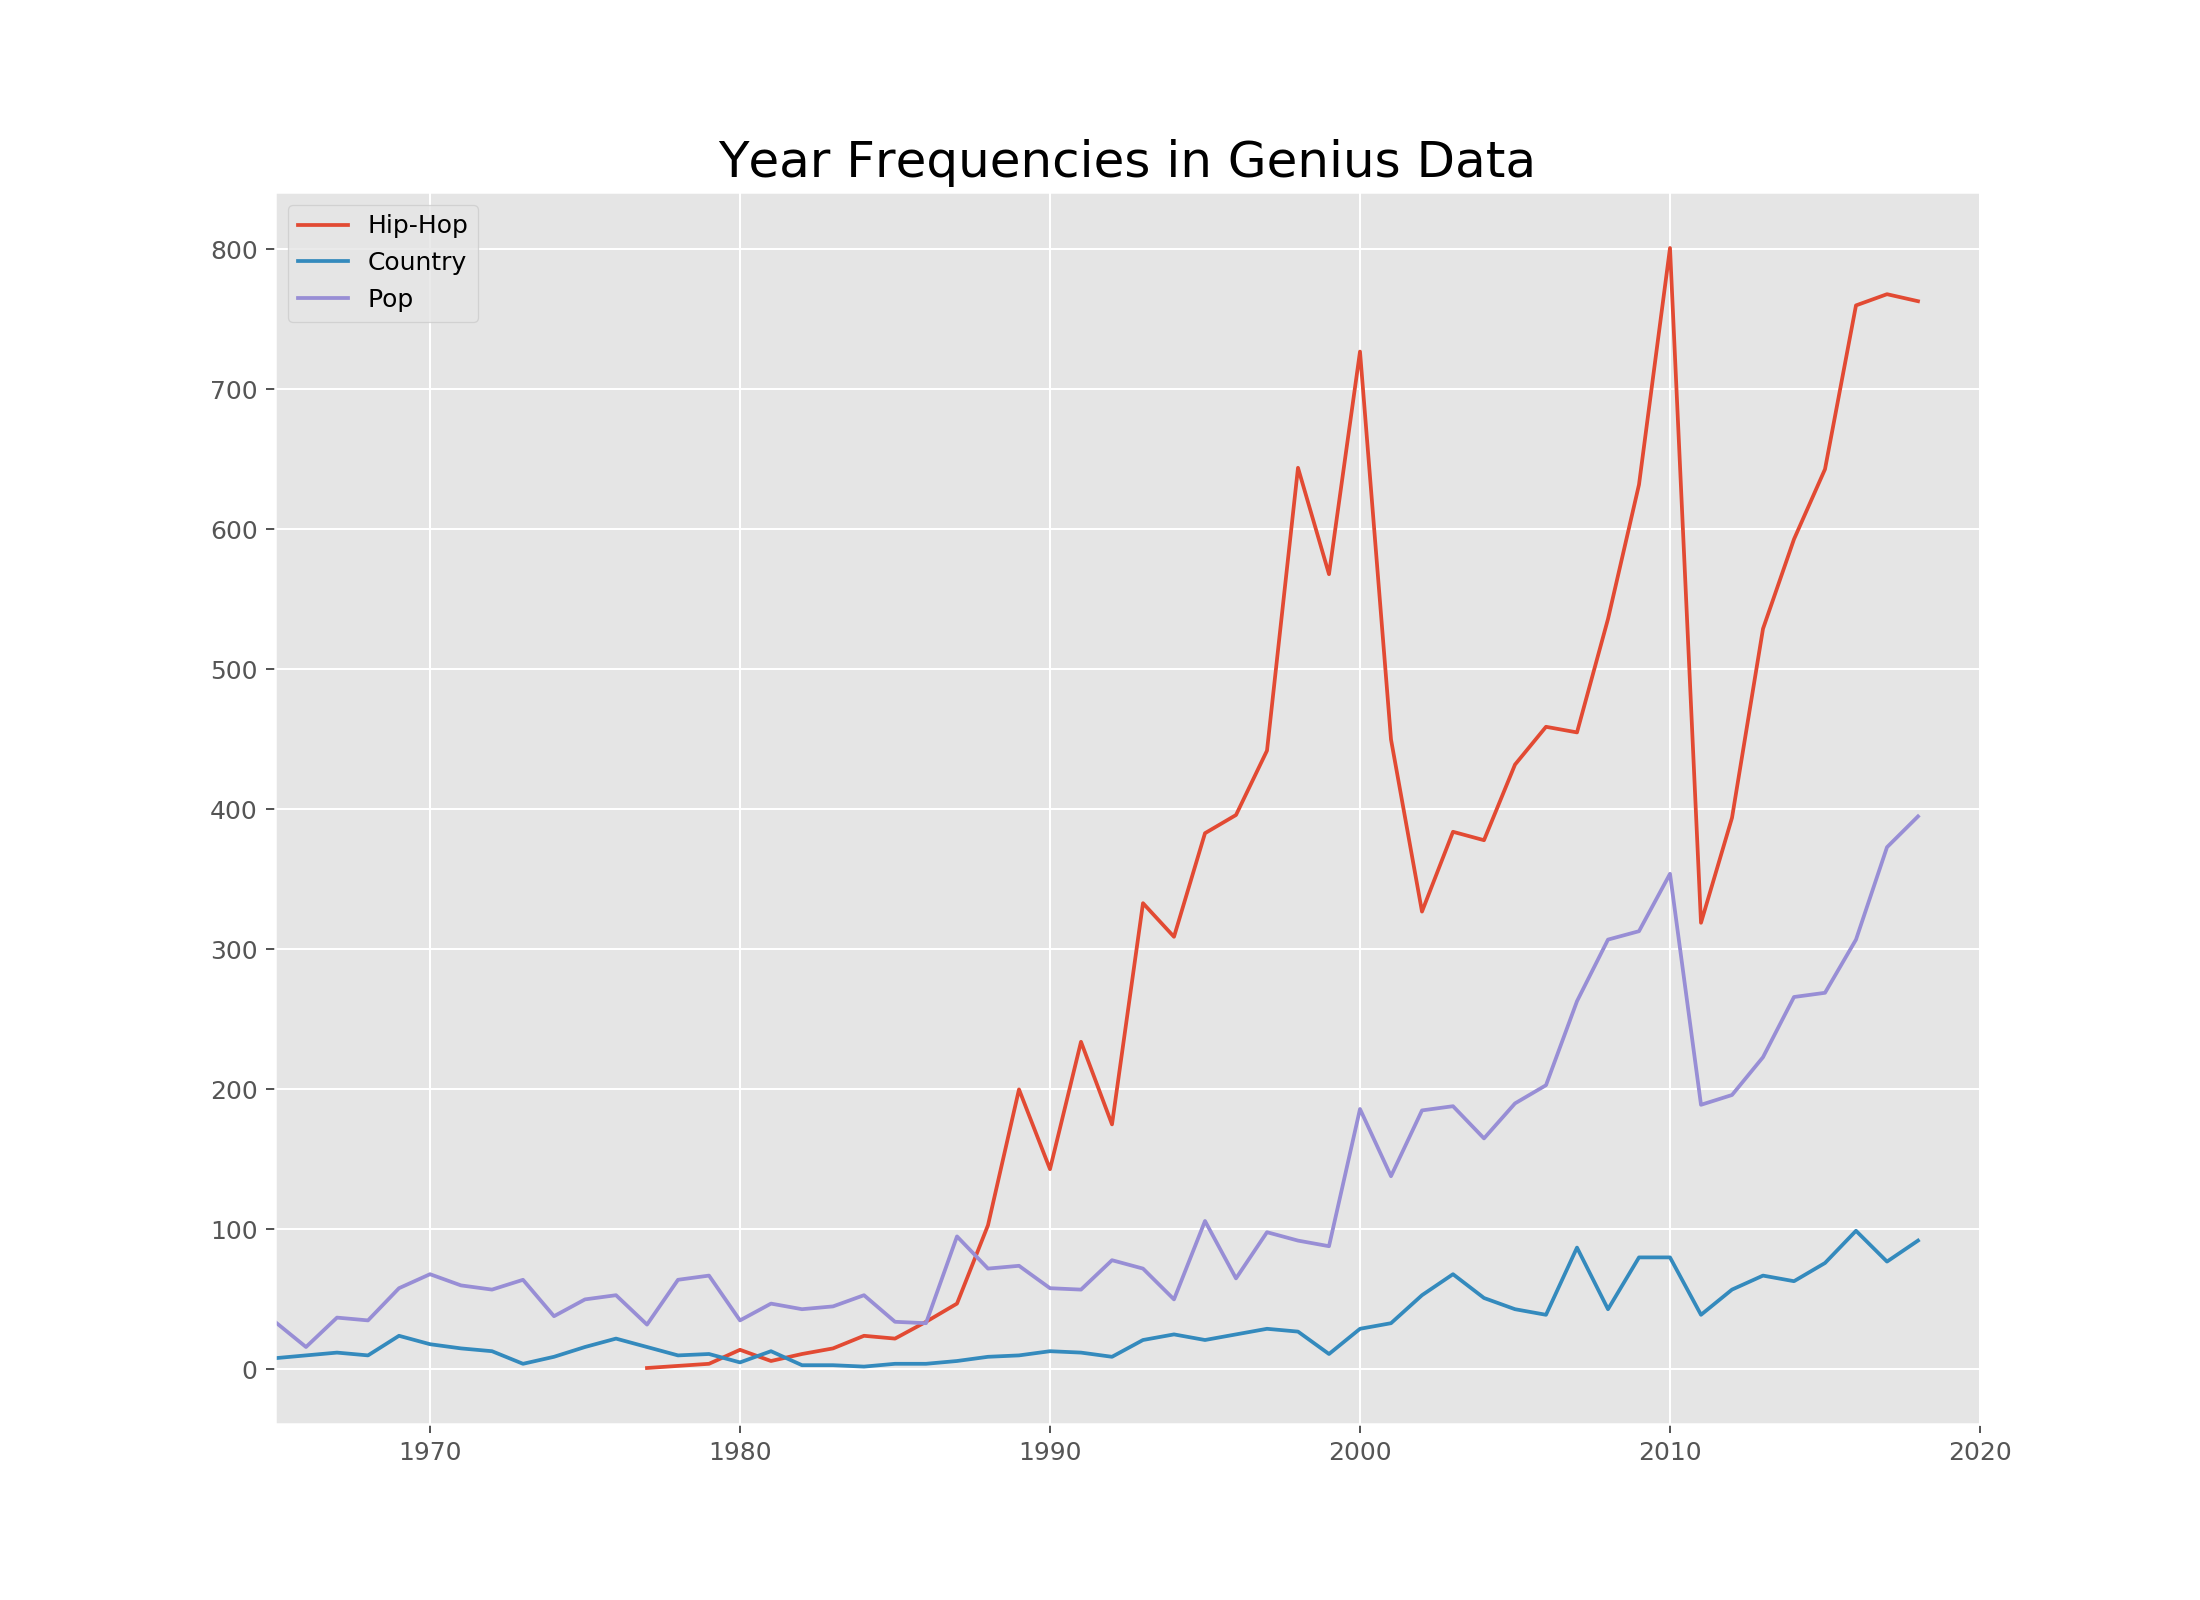
\includegraphics[width=\textwidth]{genius_histogram_line}
\caption{Frequencies in Genius Data}
\label{fig:histograms:genius}
\end{subfigure}
\begin{subfigure}[t]{0.49\textwidth}
\centering
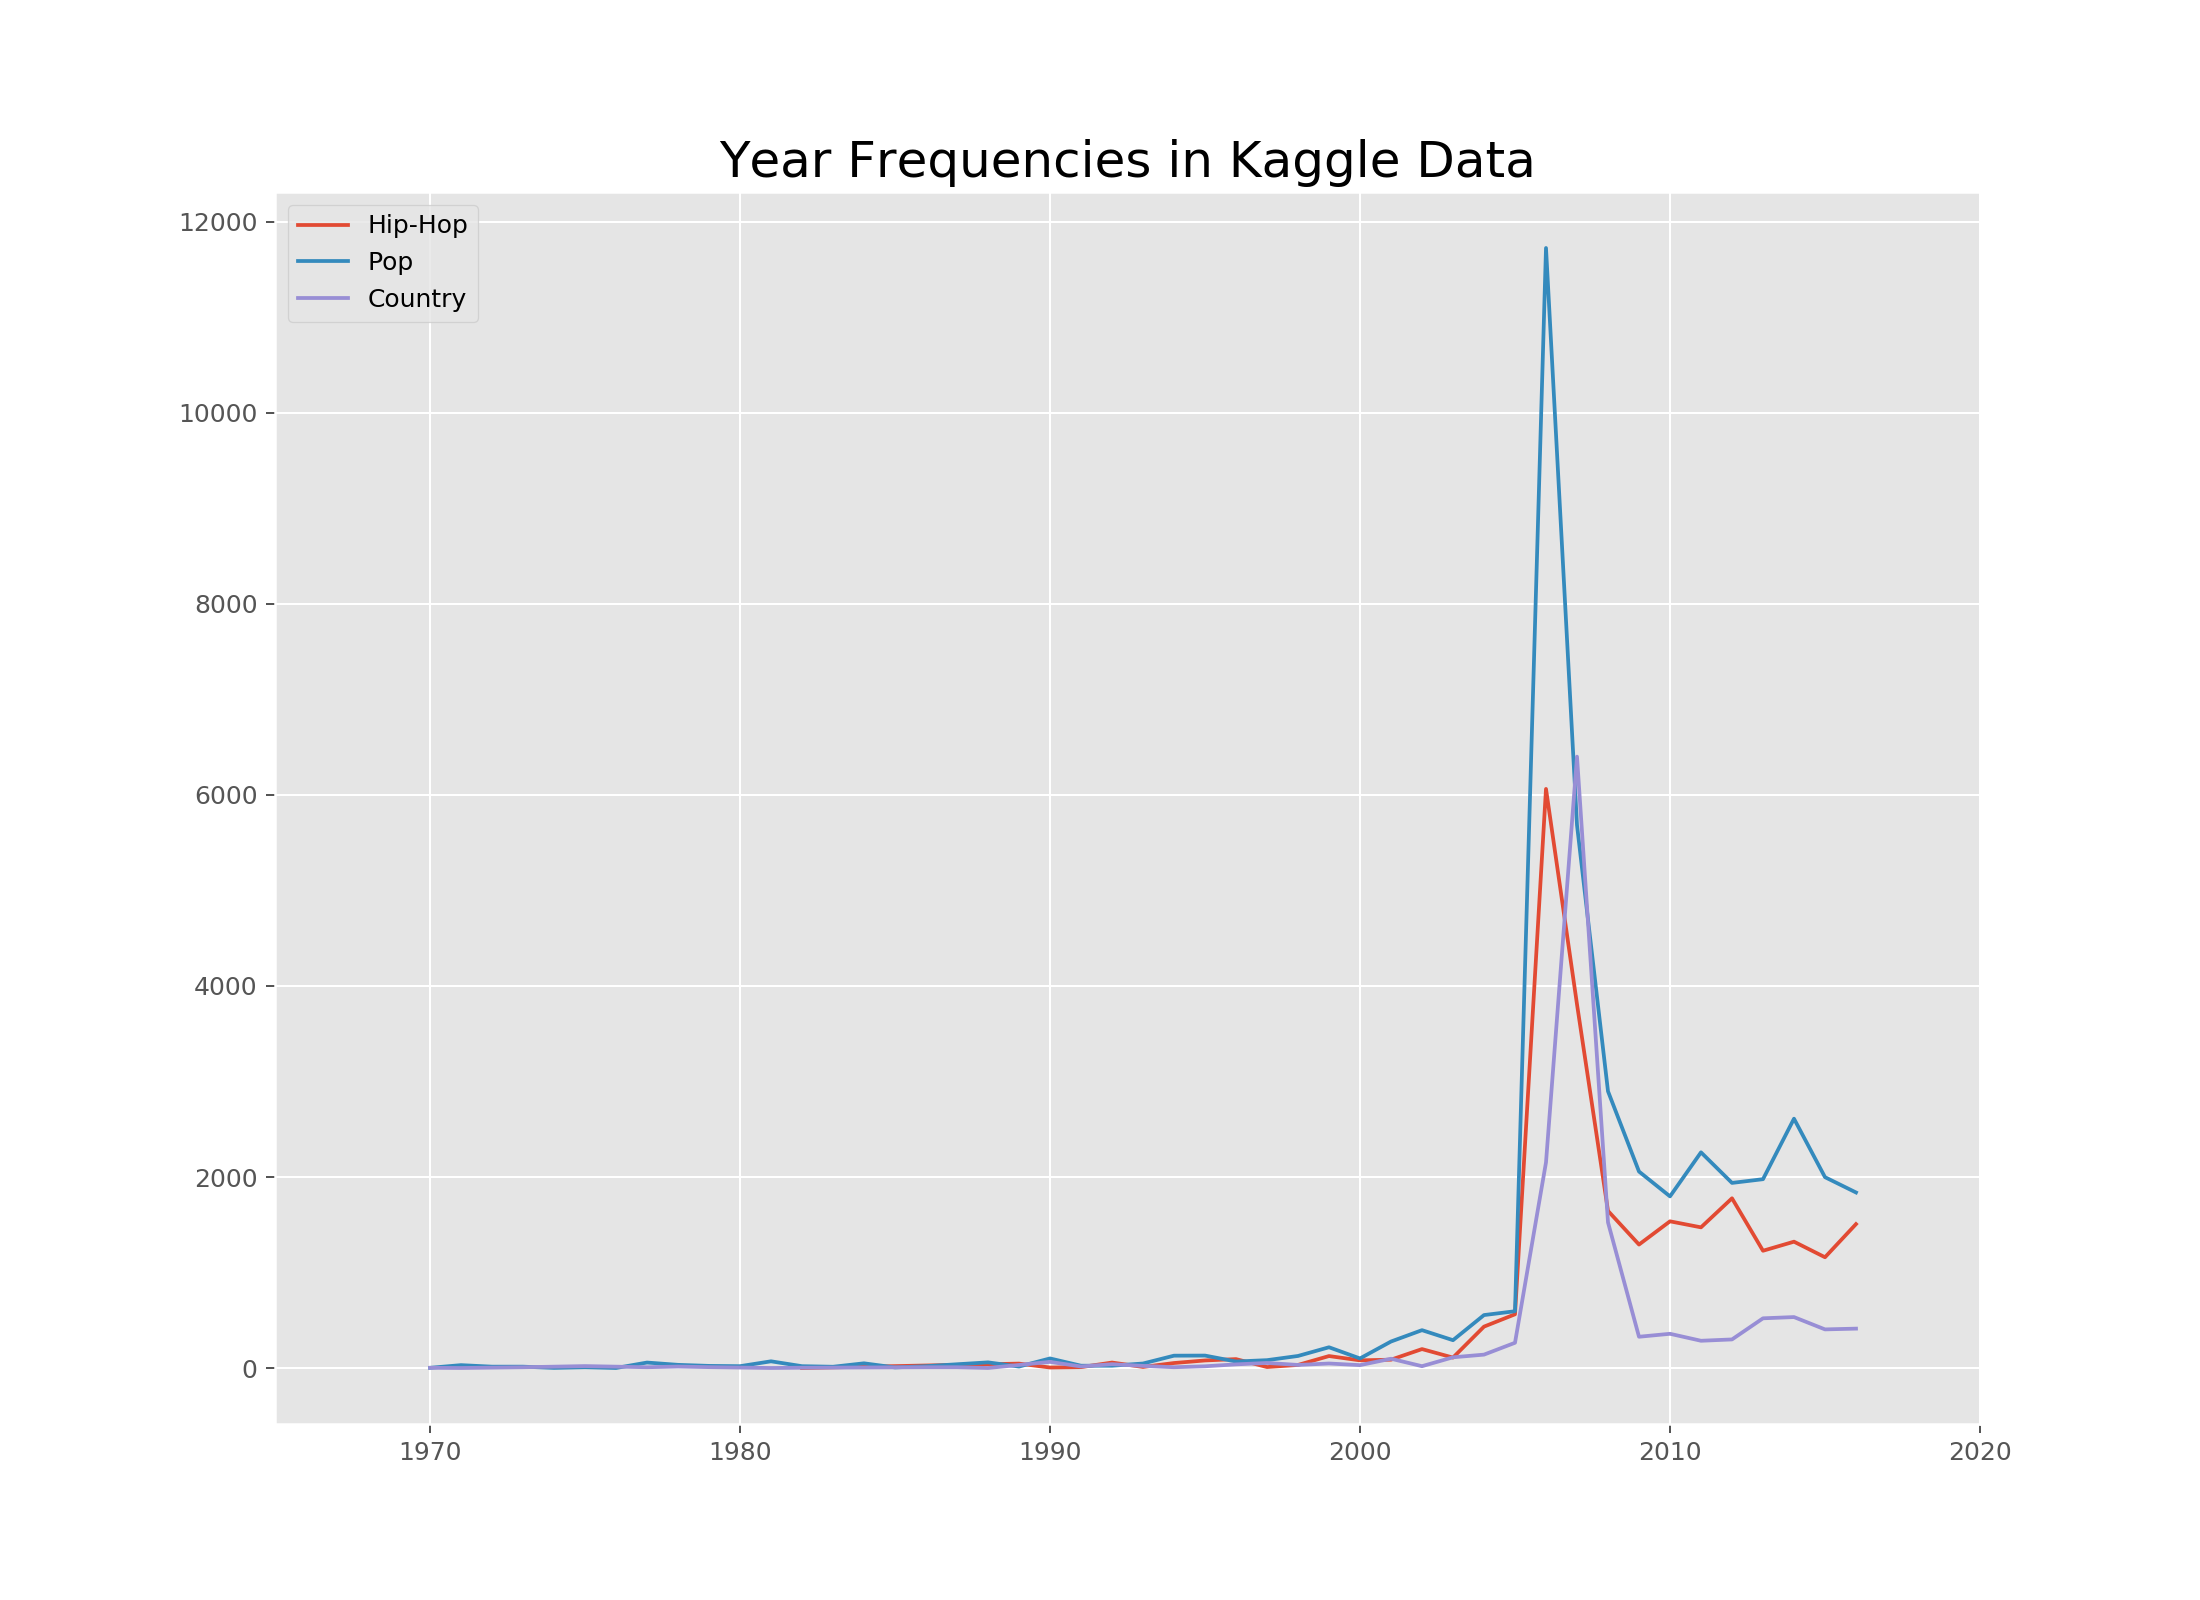
\includegraphics[width=\textwidth]{kaggle_histogram_line}
\caption{Frequencies in Kaggle Data}
\label{fig:histograms:kaggle}
\end{subfigure}
\caption{Distribution of lyrics over years}
\label{fig:histograms}
\end{figure*}
We were successful in mitigating the temporal bias the original kaggle data had. These plots show the differences between our database and kaggle respectively
\section{Reflection}

\subsection{Personal Contribution}\label{sec:contribution}
%\enquote{What did you personally contribute to the project?}

My main contribution over the whole project span was to write the scraping scripts to generate our data and take care of data management. Also, I took care of any statistics and visualizations concerning the data acquisition part. 

Besides that, I tried to make my colleagues interaction with \texttt{SQLite} as easy as possible, as they had no prior experience. From my perspective the boilerplate code I provided to construct the annotation pipeline elements helped us to create a lean and extendable annotation pipeline. However, I do not claim credits for the great pipeline elements, especially their multithreaded design.
Initially I thought I would spend more time with the individual pipeline elements. However, Atreya and Juliane had no problems handling it, so my contribution on that part was kept to package recommendation and bug fixing in one instance. 

Minor contributions included: documentation and language recognition.

\subsection{Reflection on Learning Goals}\label{sec:reflection}
% How did your project support you in obtaining your learning objectives (see planning paper)?
In this section I will discuss how our project has helped me to fulfill my learning objectives. To shortly reiterate them: 

The central goal our project was build towards was getting hands-on experience with many of the methods we discussed in class. We didn't indent to study them in-depth, rather getting acquainted with them and then continue.
Another personal learning goal was, to finally try out classifying political stance in text data, which I already wanted to do in my Bachelor's Thesis.

To begin with the latter: Unfortunately, we had to scrap the political stance analysis, since getting the lyrics took too much time and effort. I am still interested and hope to try it out soon.

\subsection{Main Take-Away and Reflection}\label{sec:takeaway}
% What are the main take-away messages from your project? What did you learn about your chosen topic?

After a while working on our project, it became rather clear that the data collection would take more time than expected. We thus parallelized the workflow. We first agreed on what data attribute we will expect from the scraped data (e.g. lyrics, year, title) and what we would annotate ourselves (e.g. sentiment valence, type token ratio). Then we could already start creating those annotation pipelines based on a small sample dataset we created for development. This approach was successful, The annotation phase only took half a day and we were able to make up for the time lost with scraping.  

One simple but important take-away I had, was to think about the structure, content and distribution of data beforehand. In earlier project the \emph{crawl first, prune later} approach was viable. In this project however it wasn't, as there is a near infinite amount of lyrics to choose from. I should have limited the number of artists per genre beforehand. The List of Country artists had 1237 even with the mentioned data loss. This introduced an significant bias afterwards, just as we originally wanted to avoid. 

Another experience I made was, that just there existing an API, doesn't make it easy, necessarily. The genius API is fairly limited, which introduced quite a number of problems. One was, that one could only query songs of a artist, given an artist id. information about genre, year or even a time span cannot be handled by the API. 
Also the responses were rather sparse. There are only few useful fields as title, artist or collaborations. The biggest problem was, that there was no data on publication year available. Also the lyrics weren't directly returned, but a link to the lyrics. Thus, we had to download the html, parse it and find the lyrics and publication year from there. 
This made it impossible to ensure the year-wise distribution beforehand. It also forced us to fully construct invalid entries, when the publication year wasn't even provided. 
To conclude the reflection, I definitely underestimated the challenge to create a custom data set. It should first be thorughly checked what an API has to offer to make sensible assumptions and also restrict the space beforehand.

% TODO: Mention git cleanup 
\section{Conclusion}\label{sec:conclusion}


% TODO: critique ego since only second person not third etc

\bibliography{../bibtex}
\bibliographystyle{acl_natbib}


%========================================================
% APPENDIX
%========================================================

\section*{Appendix}\label{sec:appendix}

\begin{figure*}
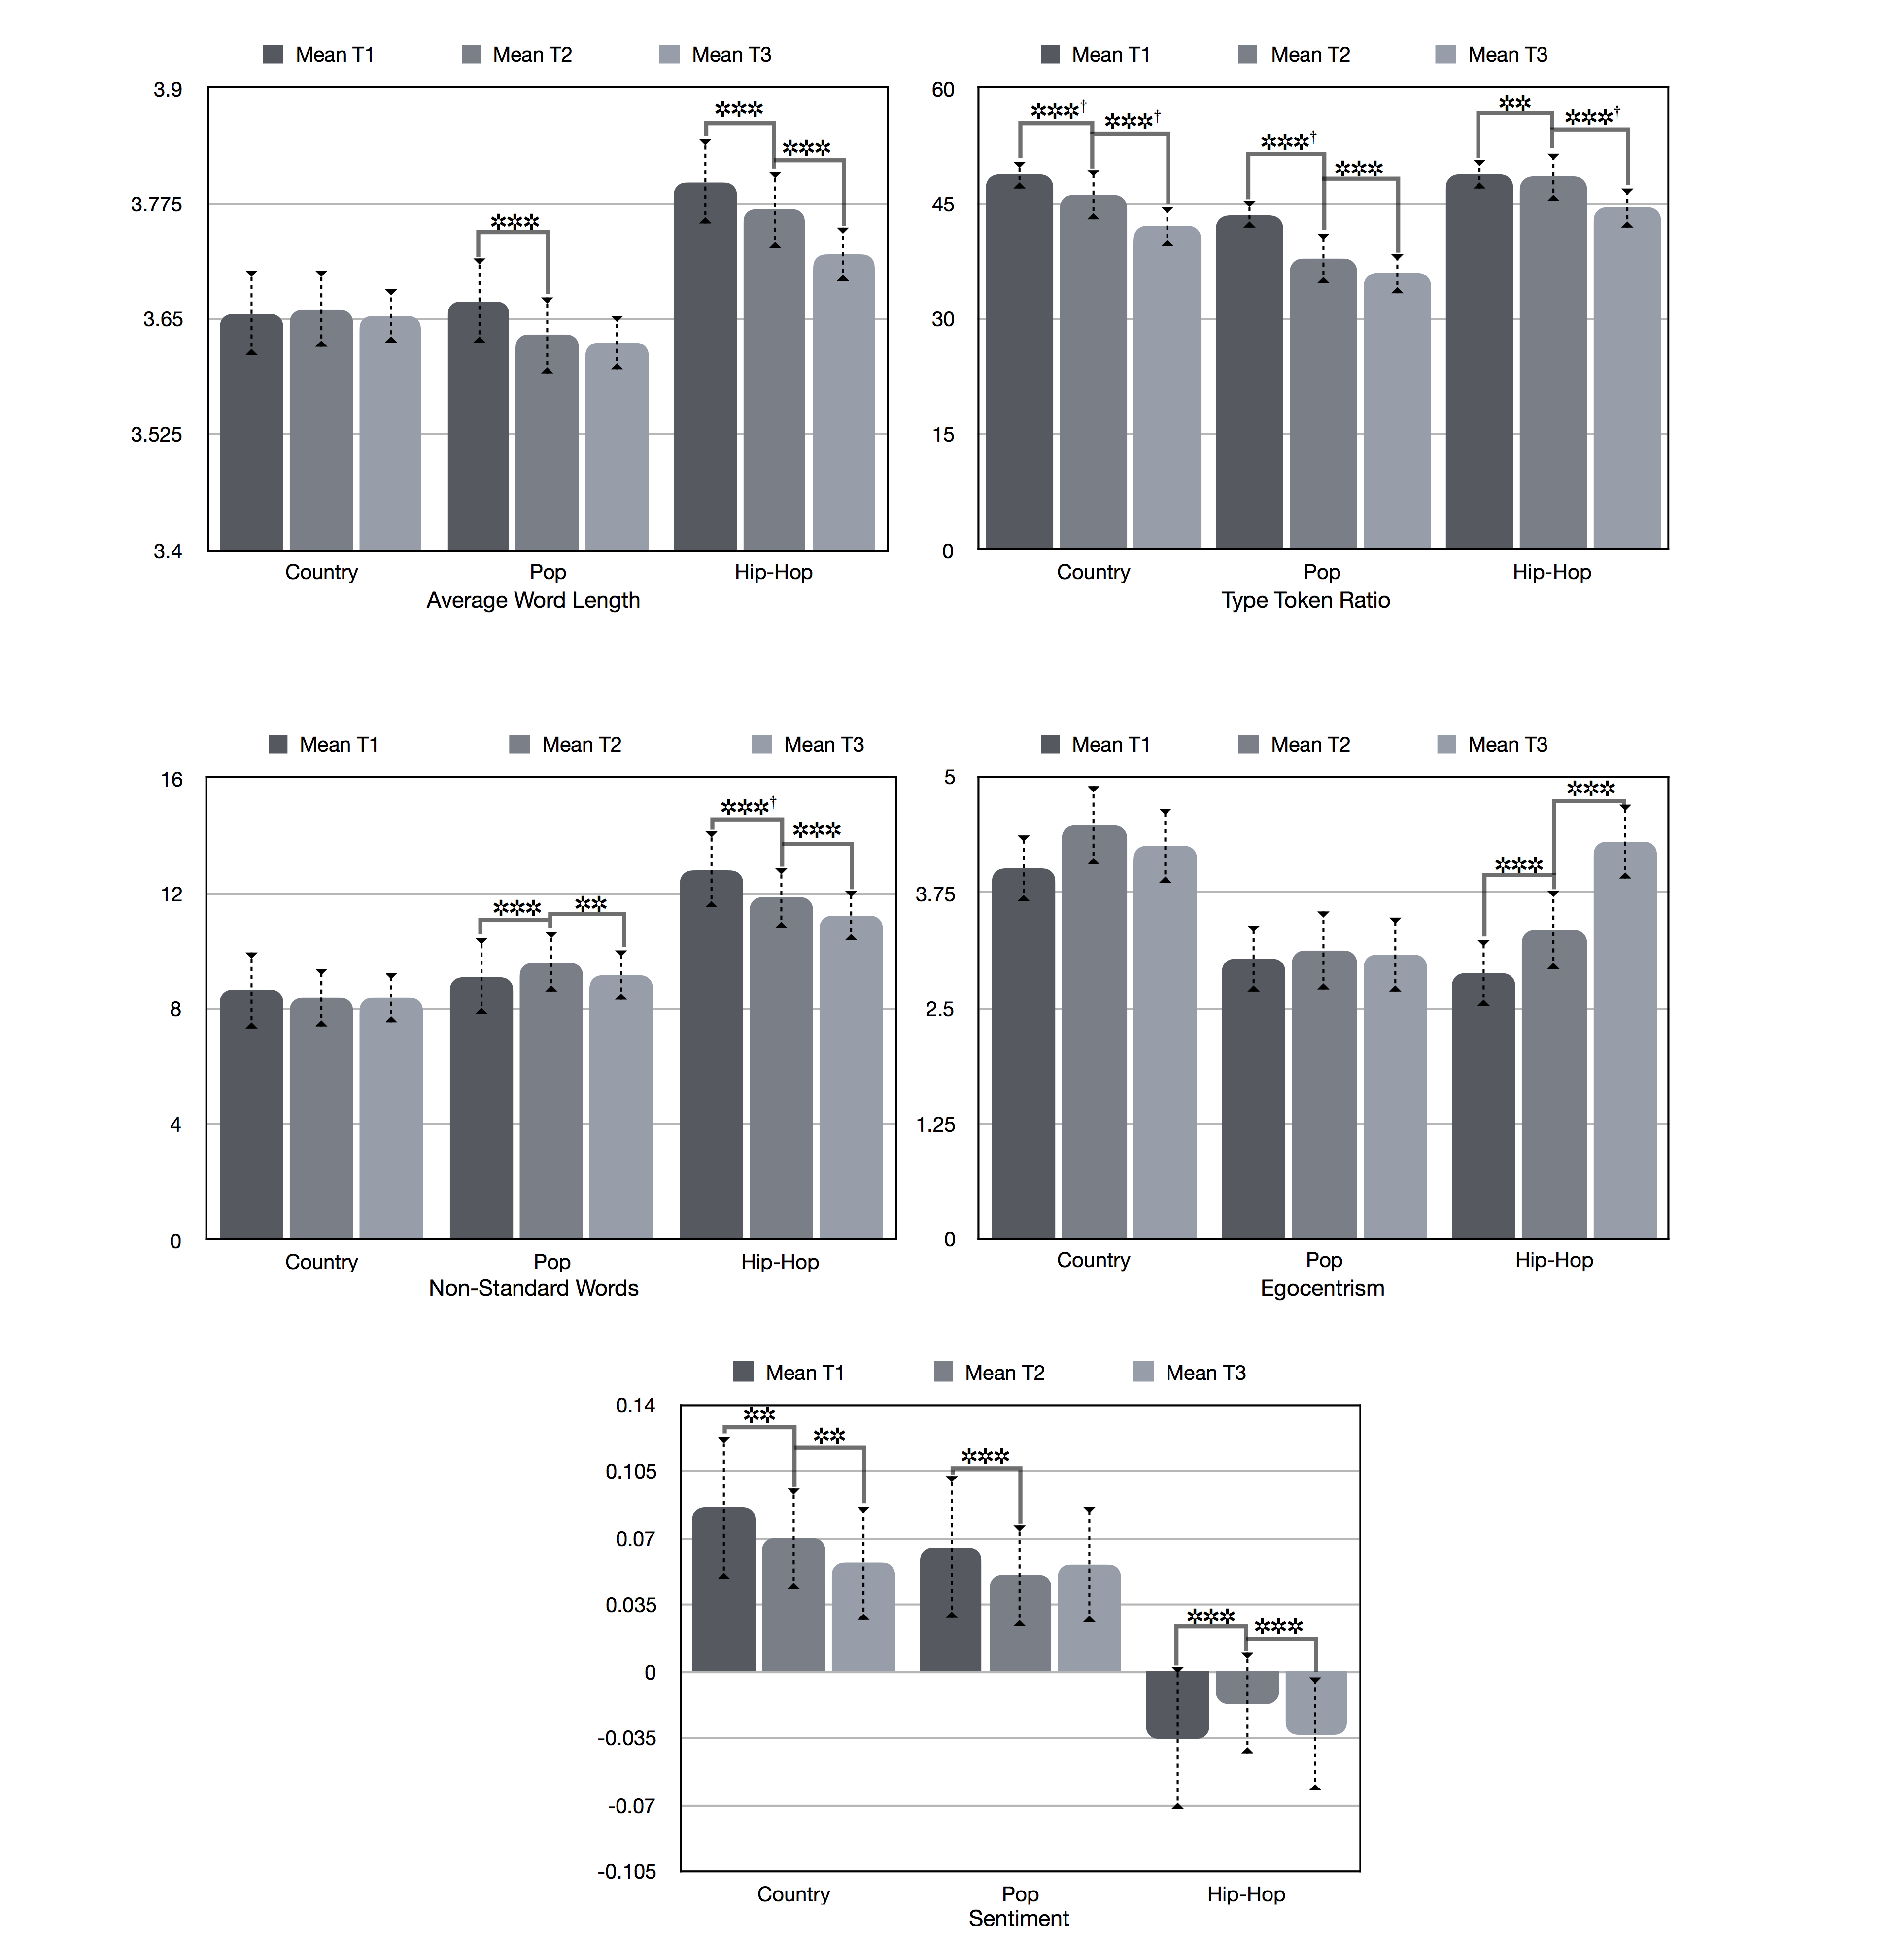
\includegraphics[width=\textwidth]{all_pvals}
\caption{p-values for all annotations.}
\label{fig:pvals}
\end{figure*}


\begin{figure*}
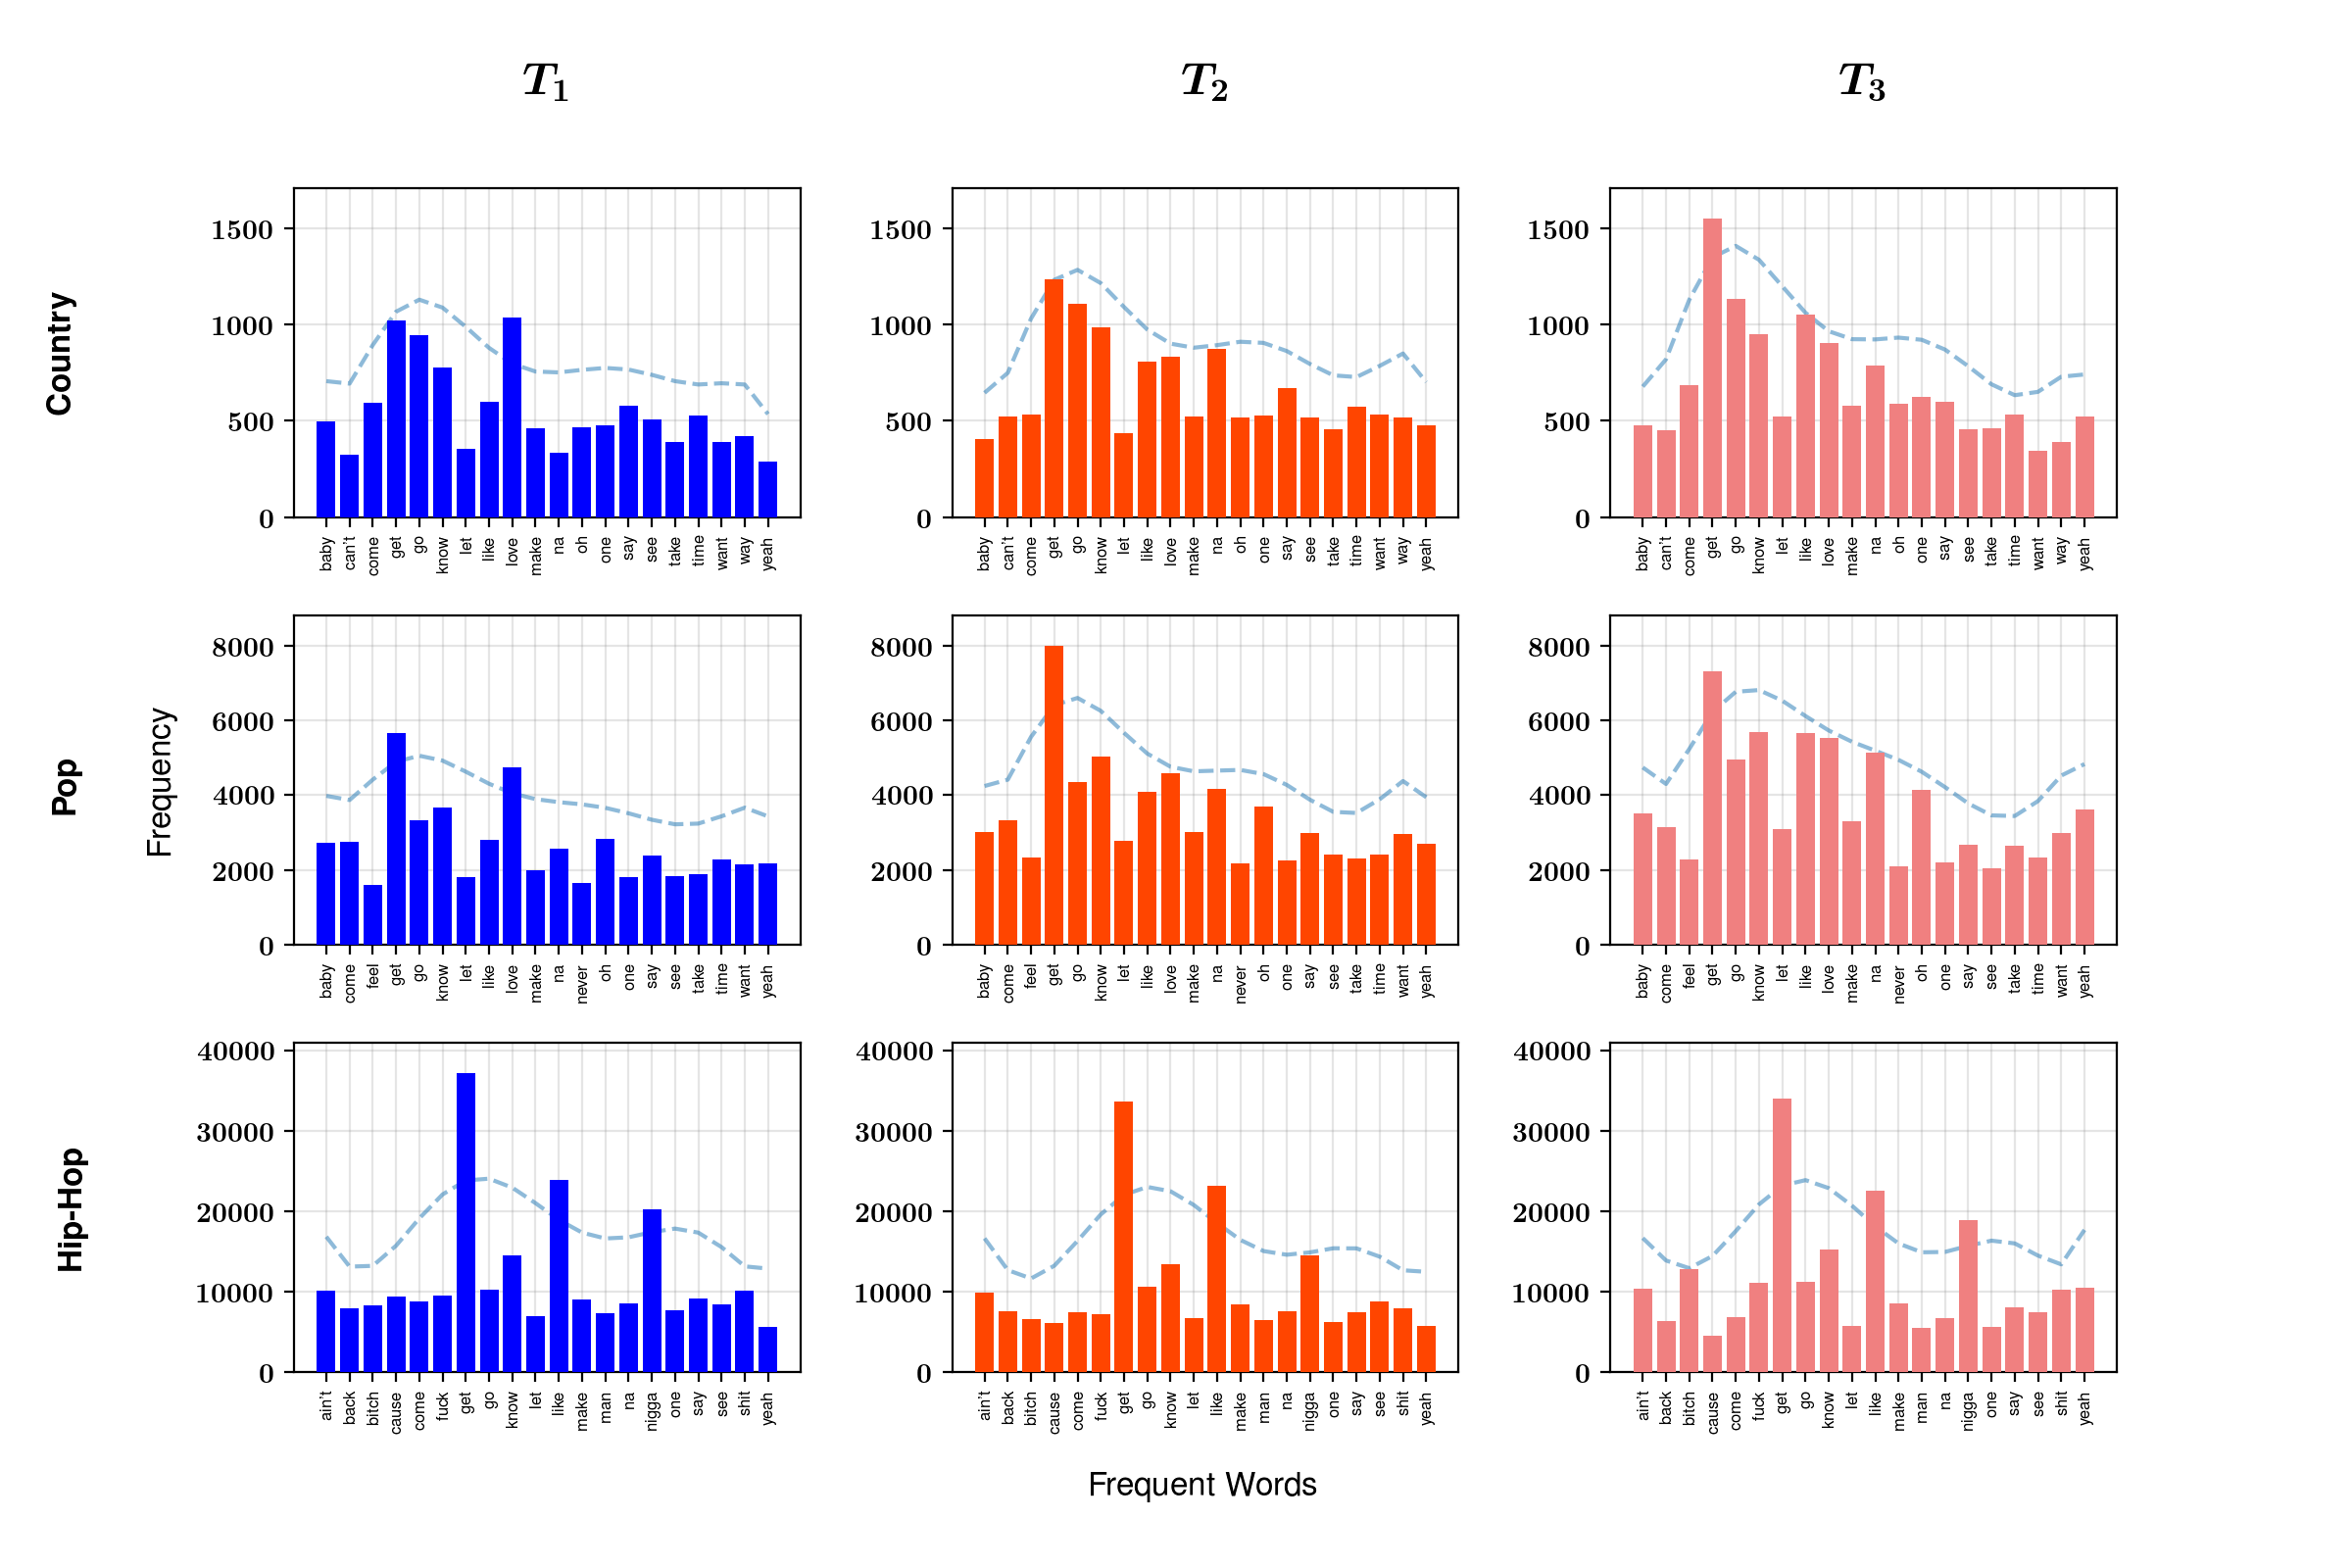
\includegraphics[width=\textwidth]{freqbarExtend}
\caption{Top 20 frequent words across data}
\label{fig:freqbarExtend}
\end{figure*}





\end{document}
